
\section{Ring-Imaging Cherenkov Detector}

% AMS RICH
In the AMS-02 experiment, the RICH is installed below the lower TOF and above the ECAL. The RICH can measure the velocity and the charge of relativistic particles. It has two kinds of radiators at its top: a sodium fluoride (NaF) radiator in the center surrounded by a silica aerogel (Agl) radiator. Below the two radiators, there is an expansion volume in the middle and a PMT plane at the bottom \cite{AMSRICHPaper1, AMSRICHPaper2}. In figure \ref{RICHDetector}, the components of the RICH are shown. The whole RICH has the shape of a cone with an upper radius of 60 cm, a lower radius of 67 cm, and a height of 47 cm. \par

% Component: Radiators and beta measurement
When a charged particle traverses a dielectric radiator with a velocity greater than the velocity of light in this material, the particle emits a cone of Cherenkov photons. By measuring the emission opening angle of the Cherenkov radiation cone $\theta = \rm{arccos} (1/n\beta)$, the $\beta$ of the particle can be obtained. The RICH in the AMS-02 experiment has a radiator plane of two non-overlapping radiators. The central radiator consists of 16 NaF tiles with a size of 85 $mm \times$ 85 $mm \times$ 5 $mm$ each and a refractive index of n=1.33. Surrounding the NaF, there are 92 silica aerogel tiles with a size of 115 $mm \times$ 115 $mm \times$ 25 $mm$ each and a refractive index of n=1.05 \cite{AMSRICHPaper1}.    \par
 
\begin{figure}[htpb]
\centering
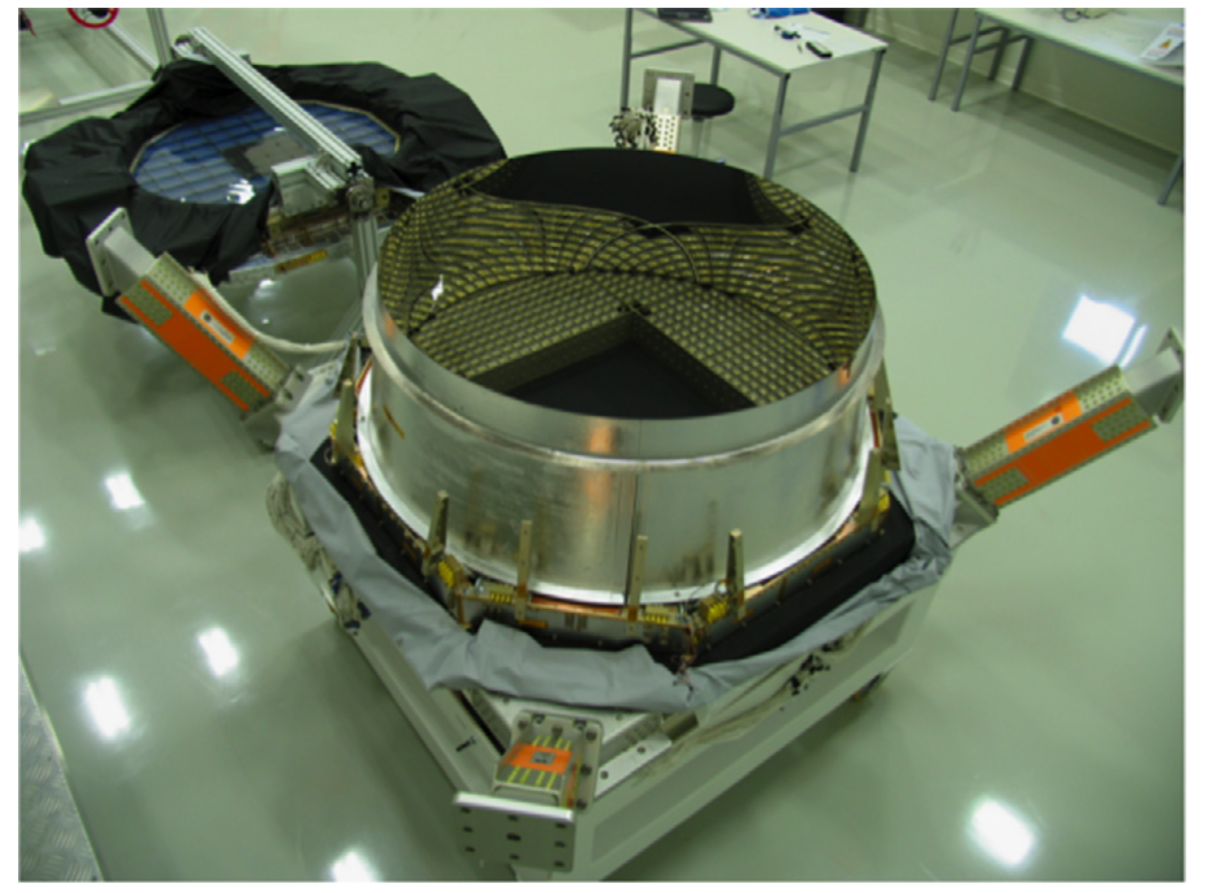
\includegraphics[width=0.8\textwidth, height=0.4\textheight ]{Figures/chapter3/RICH/RICHDetector.png}
\caption[The RICH PMT plane, its expansion volume and two radiators.]{The RICH PMT plane and its expansion volume at the front of the picture and the two radiators in the background \cite{RICHDetector}.}
\label{RICHDetector}
\end{figure}

Since $\beta=v/c$ and $n=c/v$, this leads to the requirement that particles which pass through the NaF radiator should have a velocity $\beta > 0.75$ in order to be detected, while those which pass through the Agl radiator should have a velocity $\beta > 0.953$.  \par

% Component: Expansion volume and PMT plane
\begin{figure}[H] 
\centering   
\subfigure[] { 
\label{RICHBetaResolution}    
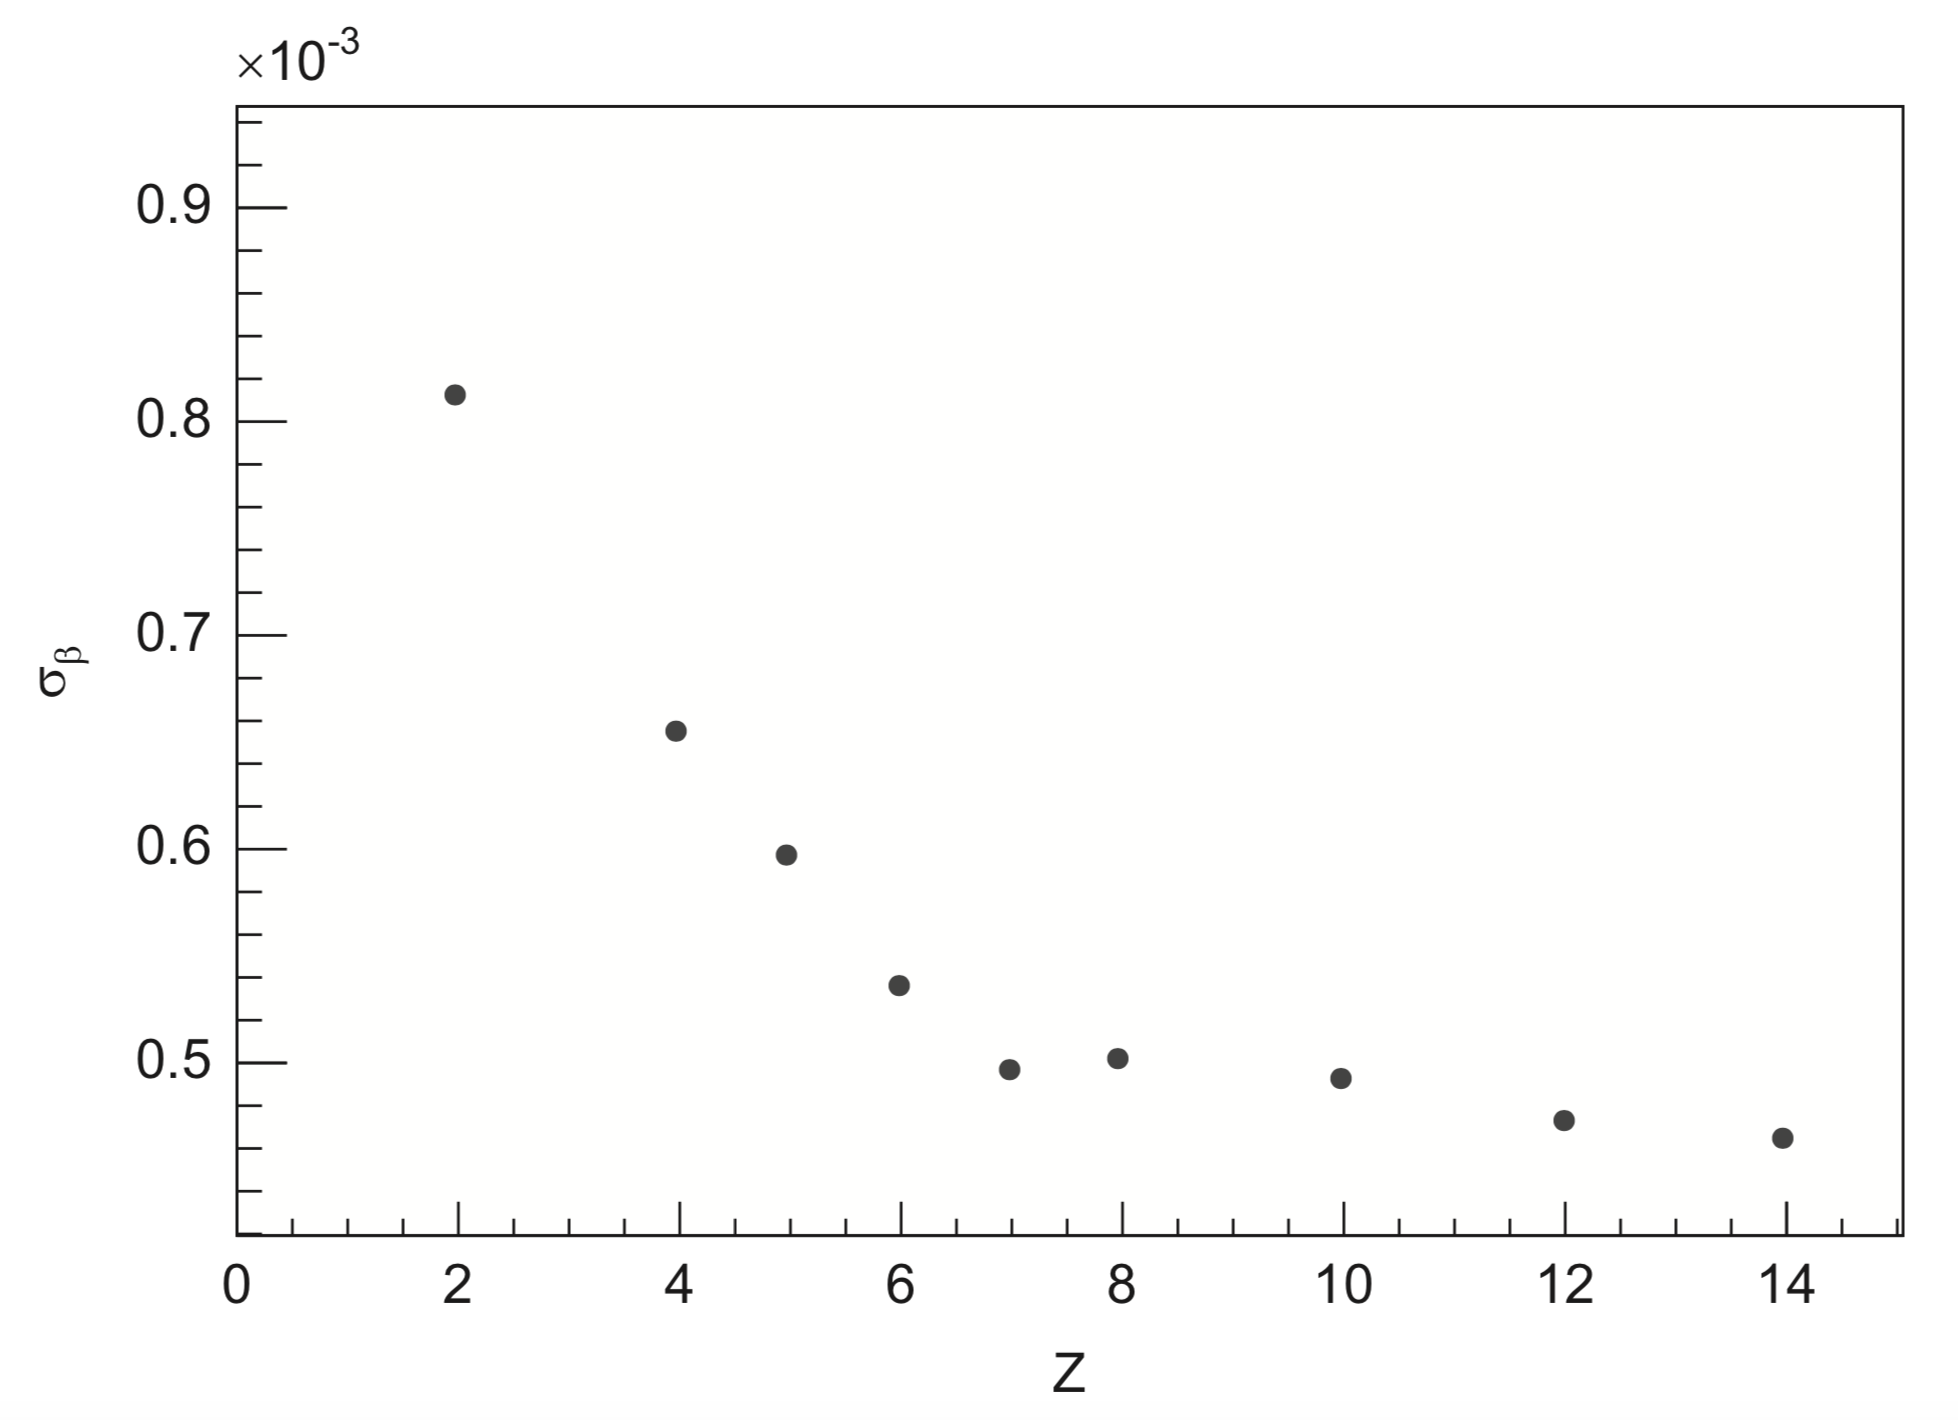
\includegraphics[width=0.45\columnwidth]{Figures/chapter3/RICH/BetaResolution.png} 
}    
\subfigure[] { 
\label{RICHChargeResolution}    
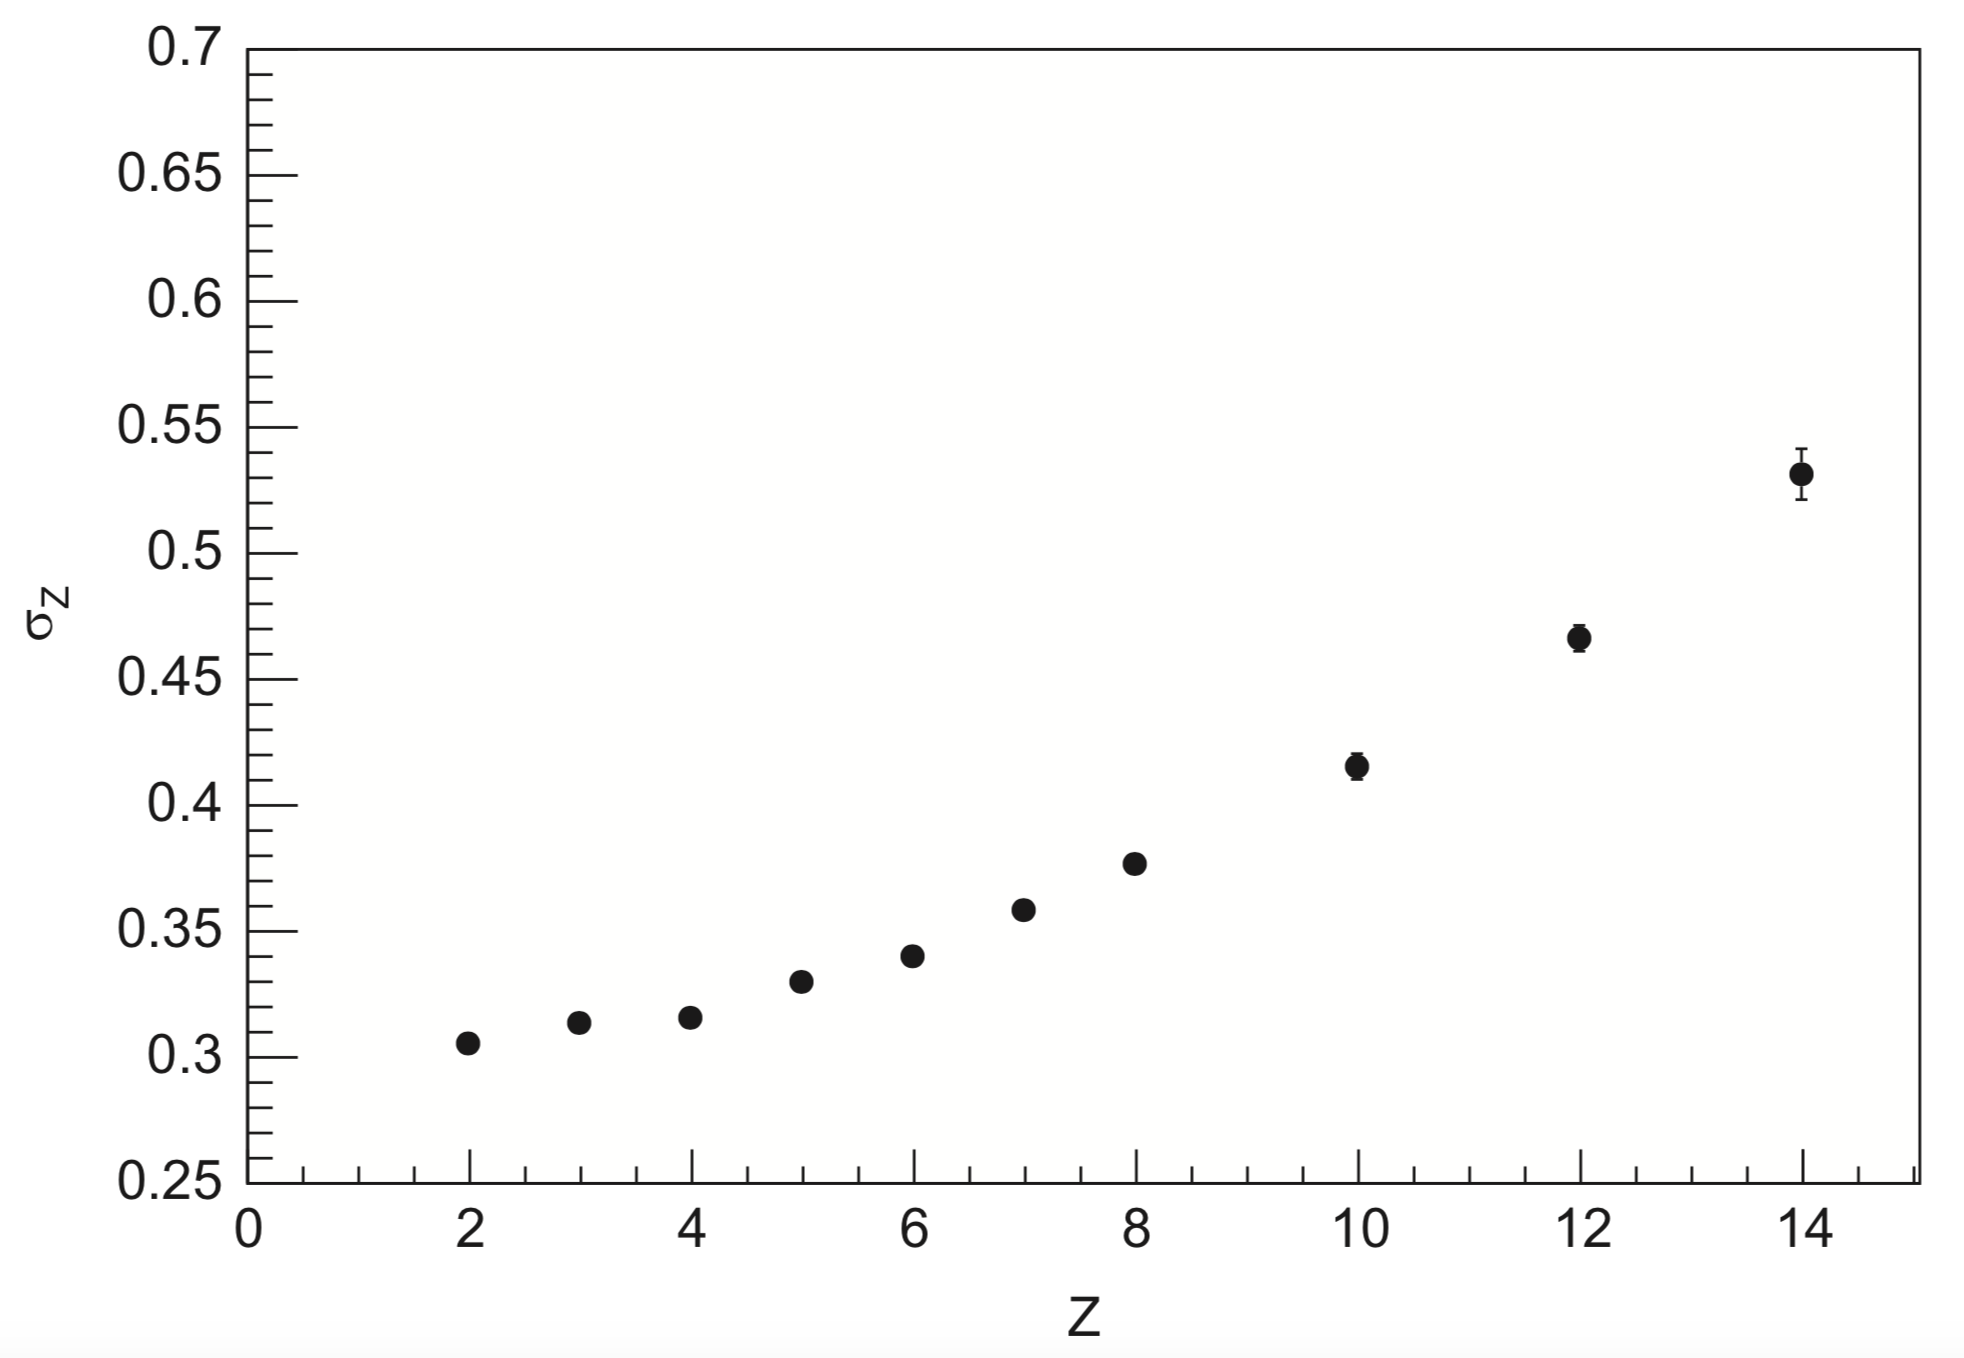
\includegraphics[width=0.45\columnwidth]{Figures/chapter3/RICH/ChargeResolution.png}    
}    
\caption[The RICH $\beta$ and charge resolution.]{a) The RICH $\beta$ resolution as a function of particle charge for the aerogel radiator \cite{RichResolution}; b) the RICH charge resolution as a function of particle charge \cite{RichResolution}.}
\end{figure}

A highly reflective mirror surrounds the expansion volume to increase the detection efficiency. The PMT detection plane at the bottom is equipped with 680 PMTs of $4 \times 4$ multi anodes. These PMTs detect the Cherenkov photons emitted in the radiators, and the effective spatial granularity is 8.5 $mm \times$ 8.5 $mm$. Since the sum of the signal amplitudes is proportional to $Z^2$, the charge of the particle can also be measured.   \par
      
% Resolutions: velocity and charge    

The velocity resolution of RICH is $\sim 10^{-3}$ for charge one particles for the aerogel radiator (figure \ref{RICHBetaResolution}). The charge measurement of RICH provides a resolution better than 0.5 for particles of charge up to 12 (figure \ref{RICHChargeResolution}).
% $\sigma_\beta / \beta \approx 10^{-3}$




